% Comprehensive test for pdfLaTeX engine
% Combines bibliography, graphics, TikZ, and advanced math
\documentclass{article}
\usepackage[utf-8]{inputenc}
\usepackage{graphicx}
\usepackage{tikz}
\usepackage{amsmath}
\usepackage{amssymb}
\usepackage{cite}

\title{Comprehensive Integration Test (pdfLaTeX)}
\author{MiKTeX Test Suite}
\date{\today}

\begin{document}

\maketitle

\section{Introduction}
This comprehensive test combines bibliography, graphics, TikZ, and advanced mathematics.

\section{Advanced Mathematics}
The Fourier transform is defined as:
\[
\hat{f}(\xi) = \int_{-\infty}^{\infty} f(x) e^{-2\pi i x \xi} dx
\]

The Cauchy-Schwarz inequality states:
\[
\left| \sum_{k=1}^{n} a_k b_k \right|^2 \leq \left( \sum_{k=1}^{n} |a_k|^2 \right) \left( \sum_{k=1}^{n} |b_k|^2 \right)
\]

\section{Graphics}
\begin{center}

\includegraphics[width=3cm]{../graphics/test-image.ppm}
\end{center}

\section{TikZ Diagram}
\begin{center}
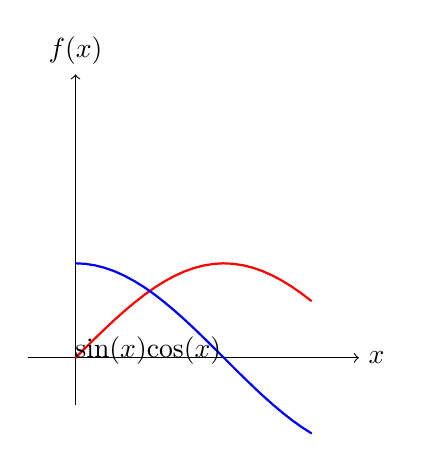
\begin{tikzpicture}[scale=1.2]
  \draw[->] (-0.5,0) -- (3,0) node[right] {$x$};
  \draw[->] (0,-0.5) -- (0,3) node[above] {$f(x)$};
  \draw[red,thick,domain=0:2.5] plot (\x, {sin(\x r)});
  \draw[blue,thick,domain=0:2.5] plot (\x, {cos(\x r)});
  \legend{$\sin(x)$, $\cos(x)$}
\end{tikzpicture}
\end{center}

\section{Bibliography}
The fundamental work by \cite{knuth1984} established TeX as a typesetting system.
Einstein's theory \cite{einstein1905} revolutionized physics.

\section{Conclusion}
All features work together seamlessly with pdfLaTeX.

\bibliography{../bibliography/references}
\bibliographystyle{plain}

\end{document}
